\documentclass[a4paper,10pt,oneside,final]{article}


\usepackage[english]{babel}
\usepackage[T1]{fontenc}
\usepackage{tabularx}
\usepackage[usenames,dvipsnames]{color}
\usepackage[table]{xcolor}
\usepackage[left=3.0cm, right=2.5cm, top=2.5cm, bottom=2.5cm]{geometry}
\usepackage{graphicx}
\usepackage{float}
\usepackage{caption}
\usepackage{listings}




\lstdefinestyle{ccc} 
{ 
numbers=none, 
basicstyle=\ttfamily, 
keywordstyle=\bf\color[RGB]{0,0,255}, 
commentstyle=\color[RGB]{178,34,34}, 
stringstyle=\color[rgb]{0.627,0.126,0.941}, 
backgroundcolor=\color{white}, 
frame=tb, %frame= lrtb, 
framerule=0.5pt, 
linewidth=\textwidth,
%aboveskip=-4.0pt,
%belowskip=-4.0pt,
lineskip=-5.0pt,
}

%
% Define author(s) and  component's name
%
\def\defauthor{Lasse Lehtonen}
\def\deftitle{HIBI\_PE\_DMA\\Reference Manual}



\author{\defauthor}
\title{\deftitle}

\usepackage{fancyhdr} 
\pagestyle{fancy} 
\lhead{\bfseries Department of Computer Systems\\
  Faculty of Computing and Electrical Engineering}
\chead{} 
\rhead{\bfseries \deftitle} 
\lfoot{\thepage} 
\cfoot{}
\rfoot{
\includegraphics[height=1.0cm]{pic/tty_logo.png}}
%\renewcommand{\headrulewidth}{0.4pt}
%\renewcommand{\footrulewidth}{0.4pt}

%\setlength{\headheight}{\headheight+1cm}
%\setlength{\textheight}{\textheight-2cm}
%\setlength{\footskip}{\footskip+1cm}

\def\deftablecolora{blue!10!white}
\def\deftablecolorb{white}


\begin{document}



%\maketitle
%\thispagestyle{empty}

\begin{titlepage}
\begin{center}

\vspace{6.0cm}
\textsc{\LARGE Tampere University of Technology}\\[1.0cm]
\textsc{\Large Faculty of Computing and Electrical Engineering}\\[1.0cm]
\textsc{\Large Department of Computer Systems}\\[1.0cm]
\vspace{6.0cm}
\hrule
\vspace{0.4cm}
{ \huge \bfseries HIBI\_PE\_DMA\\\vspace{10pt}HW Reference Manual}
\vspace{0.4cm}
\hrule

%\vspace{2.0cm}

\vfill

\begin{minipage}{0.4\textwidth}
\begin{flushleft} \large
\emph{Author:}\\
\defauthor
\end{flushleft}
\end{minipage}
\begin{minipage}{0.4\textwidth}
\begin{flushright} \large
\emph{Updated:} \\
\today
\end{flushright}
\end{minipage}

\end{center}
\end{titlepage}

\newpage
\tableofcontents



\newpage
\section{REVISION HISTORY}
\setcounter{page}{1}

\begin{center}
  \rowcolors{3}{\deftablecolora}{\deftablecolorb}
  
  \captionof{table}{}
  \begin{tabularx}{\textwidth}{|lllX|}
    \hline
    Revision & Author          & Date    & Description\\
    \hline
    1.03  & Lasse Lehtonen  & 26.01.2012 & Ported old document to Latex\\
    1.04  & Lasse Lehtonen  & 27.01.2012 & Added streaming channels\\
    1.05  & Lasse Lehtonen  & 02.03.2012 & Removed SW part and changed register order\\
    & & & \\
    & & & \\
    \hline
  \end{tabularx}
\end{center}



\newpage
\section{DOCUMENT OVERVIEW}

\subsection{SCOPE}

This documentation describes how to use HIBI PE DMA component.

\subsection{AUDIENCE}

For hardware integrators and software developers using this component.

\subsection{RELATED DOCUMENTATION}

\begin{center}
  \rowcolors[]{2}{\deftablecolora}{\deftablecolorb}

  \captionof{table}{}
  \begin{tabularx}{\textwidth}{|lX|}
    \hline
    Document & Description\\
    \hline    
    building\_test\_system.pptx & Descibes an example using in SOPC 
                                  with NIOS II processors\\
    hpd\_sw\_ref.pdf   & Software reference manual\\
    HIBI\_PE\_DMA.pptx & Introduction to HIBI PE DMA\\
    \hline
  \end{tabularx}
\end{center}

\subsection{DOCUMENT CONVENTIONS}


\begin{itemize}
\item Ports: \texttt{teletype} in text
\item Generics: \texttt{teletype} in text
\end{itemize}



\newpage
\section{INTRODUCTION}

\subsection{BRIEF DESCRIPTION}

HIBI\_PE\_DMA (HPD) component allows separate processor systems with
Avalon-MM compatible interface to communicate with each other via Hibi
hierarchical bus. Communication is DMA based and uses either packet or
stream channels for network transactions. HIBI\_PE\_DMA supports both
polling and interrupts.

\subsection{EXAMPLE SYSTEM}

Example system showing three SOPC blocks with Nios processors
communicating via Hibi. Each HIBI\_PE\_DMA component is associated
with dual-port RAMs where they store received data and read the data
to be sent.

\begin{center}  
  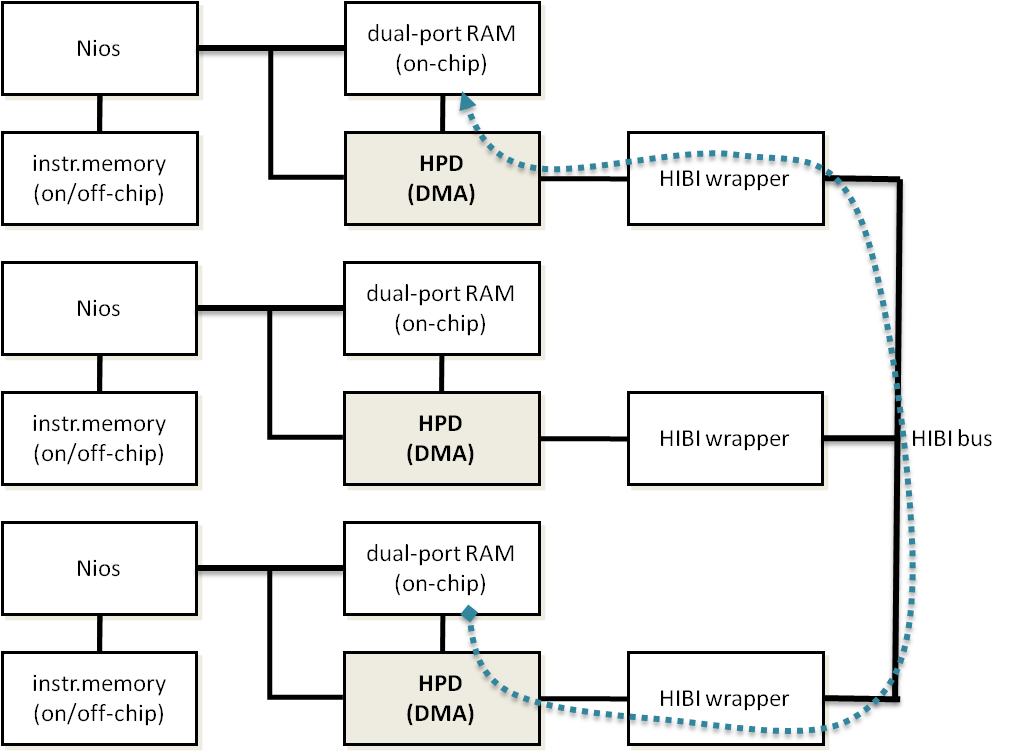
\includegraphics[width=0.8\textwidth]{pic/example_system.png}
  \captionof{figure}{Example system with three Nios processors}  
  \label{fig:example_system}
\end{center}



\newpage
\section{HARDWARE DESIGN}

\subsection{HIBI\_PE\_DMA}

\subsubsection{GENERICS}

\begin{center}
  \rowcolors{3}{\deftablecolora}{\deftablecolorb}

  \captionof{table}{}
  \begin{tabularx}{\textwidth}{|lX|}
    \hline
    Name                   & Description\\
    \hline
    data\_width\_g         & Width of the data buses\\
    addr\_width\_g         & Width of the Hibi address\\
    words\_width\_g        & Number of bits needed to represent word counters\\
    n\_stream\_chans\_g    & Number of stream channels\\
    n\_packet\_chans\_g    & Number of packet channels\\
    n\_chans\_bits\_g      & Bits needed to represent n\_stream\_chans\_g + 
                             n\_packet\_chans\_g\\
    hibi\_addr\_cmp\_lo\_g & Lower boundary for address comparison\\
    hibi\_addr\_cmp\_hi\_g & Upper boundary for address comparison\\
    \hline
  \end{tabularx}
\end{center}

\subsubsection{CLOCKING AND RESET}

\begin{center}
  \rowcolors{3}{\deftablecolora}{\deftablecolorb}

  \captionof{table}{}
  \begin{tabularx}{\textwidth}{|lllX|}
    \hline
    Port   & Width & Direction & Description\\
    \hline
    clk    & 1     & in        & Clock, active on rising edge\\
    rst\_n & 1     & in        & Reset, asynchronous, active low\\
    \hline
  \end{tabularx}
\end{center}



\subsubsection{CONFIGURATION INTERFACE}

This slave interface is used by the processor for reading or writing
HIBI\_PE\_DMA registers.

\begin{center}
  \rowcolors{3}{\deftablecolora}{\deftablecolorb}

  \captionof{table}{}
  \begin{tabularx}{\textwidth}{|lllX|}
    \hline
    Port   & Width & Direction & Description\\
    \hline
    avalon\_cfg\_addr\_in         & n\_chans\_g+4  & in  & Register address\\
    avalon\_cfg\_writedata\_in    & addr\_width\_g & in  & Data in\\
    avalon\_cfg\_we\_in           & 1              & in  & Write enable\\
    avalon\_cfg\_readdata\_out    & addr\_width\_g & out & Data out\\
    avalon\_cfg\_re\_in           & 1              & in  & Read enable\\
    avalon\_cfg\_cs\_in           & 1              & in  & Chip select\\
    avalon\_cfg\_waitrequest\_out & 1              & out & Stall\\
    \hline
  \end{tabularx}
\end{center}


\subsubsection{MEMORY WRITE INTERFACE}

This master interface is used by HIBI\_PE\_DMA to write received data to the
shared dual-port memory.

\begin{center}
  \rowcolors{3}{\deftablecolora}{\deftablecolorb}

  \captionof{table}{}
  \begin{tabularx}{\textwidth}{|lllX|}
    \hline
    Port   & Width & Direction & Description\\
    \hline
    avalon\_addr\_out\_rx       & addr\_width\_g     & out & Write address\\
    avalon\_we\_out\_rx         & 1                  & out & Write enable\\
    avalon\_be\_out\_rx         & data\_width\_g / 8 & out & Byte enable\\
    avalon\_writedata\_out\_rx  & data\_width\_g     & out & Data out\\
    avalon\_waitrequest\_in\_rx & 1                  & in  & Stall\\
    \hline
  \end{tabularx}
\end{center}

\pagebreak
\subsubsection{MEMORY READ INTERFACE}

This master interface is used by HIBI\_PE\_DMA to read data to be sent from the
shared dual-port memory.

\begin{center}
  \rowcolors{3}{\deftablecolora}{\deftablecolorb}

  \captionof{table}{}
  \begin{tabularx}{\textwidth}{|lllX|}
    \hline
    Port   & Width & Direction & Description\\
    \hline
    avalon\_addr\_out\_tx         & addr\_width\_g & out & Read address\\
    avalon\_re\_out\_tx           & 1              & out & Read enable\\
    avalon\_readdata\_in\_tx      & data\_width\_g & in  & Data in\\
    avalon\_waitrequest\_in\_tx   & 1              & in  & Stall\\
    avalon\_readdatavalid\_in\_tx & 1              & out & Byte enable\\
    \hline
  \end{tabularx}
\end{center}


\subsubsection{HIBI RECEIVE INTERFACE}

\begin{center}
  \rowcolors{3}{\deftablecolora}{\deftablecolorb}

  \captionof{table}{}
  \begin{tabularx}{\textwidth}{|lllX|}
    \hline
    Port   & Width & Direction & Description\\
    \hline
    hibi\_data\_in  & data\_width\_g & in  & Data in\\
    hibi\_av\_in    & 1              & in  & Address valid\\
    hibi\_empty\_in & 1              & in  & No more data\\
    hibi\_comm\_in  & 5              & in  & Hibi command\\
    hibi\_re\_out   & 1              & out & Read enable\\
    \hline
  \end{tabularx}
\end{center}


\subsubsection{HIBI TRANSMIT INTERFACE}

\begin{center}
  \rowcolors{3}{\deftablecolora}{\deftablecolorb}

  \captionof{table}{}
  \begin{tabularx}{\textwidth}{|lllX|}
    \hline
    Port   & Width & Direction & Description\\
    \hline
    hibi\_data\_out & data\_width\_g & in  & Data out\\
    hibi\_av\_out   & 1              & in  & Address valid\\
    hibi\_full\_in  & 1              & in  & Receiver fulll\\
    hibi\_comm\_out & 5              & in  & Hibi command\\
    hibi\_we\_out   & 1              & out & Write enable\\
    \hline
  \end{tabularx}
\end{center}


\subsubsection{INTERRUPT INTERFACE}

\begin{center}
  \rowcolors{3}{\deftablecolora}{\deftablecolorb}

  \captionof{table}{}
  \begin{tabularx}{\textwidth}{|lllX|}
    \hline
    Port   & Width & Direction & Description\\
    \hline
    rx\_irq\_out & 1 & out  & Interrupt, active high\\
    \hline
  \end{tabularx}
\end{center}


\pagebreak
\subsubsection{INTERFACE STRUCTURE}

Figure \ref{fig:arch} shows how HIBI\_PE\_DMA's interfaces are connected.

\begin{center}  
  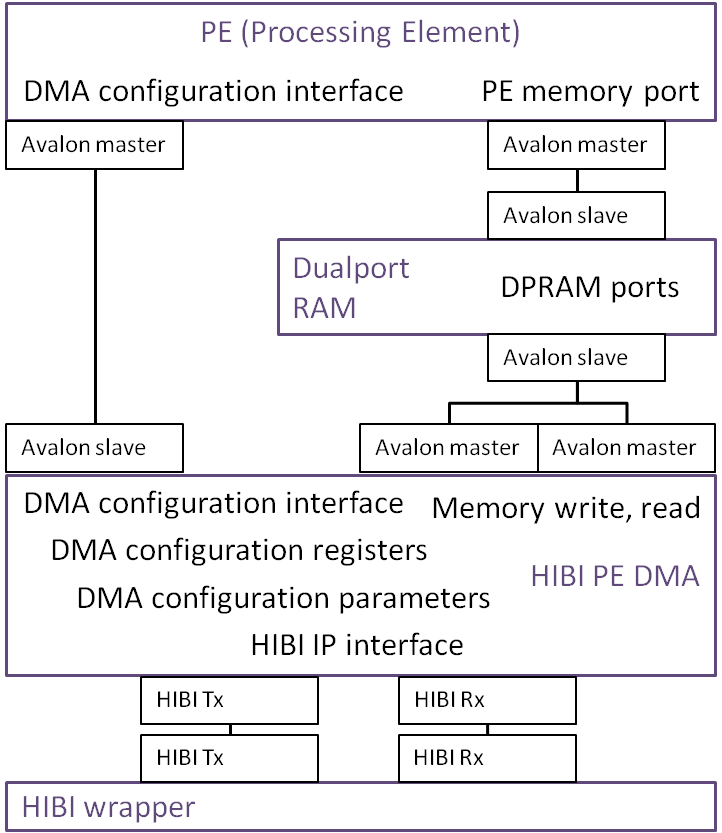
\includegraphics[width=0.8\textwidth]{pic/arch.png}
  \captionof{figure}{HIBI\_PE\_DMA connected to a Processing Element
    (PE), dual-port memory and Hibi}
  \label{fig:arch}
\end{center}


\subsubsection{INTEGRATION}

Related  source  files  are listed  in  next  table  in the  order  of
compilation (when applicable).

\begin{center}
  \rowcolors{3}{\deftablecolora}{\deftablecolorb}

  \captionof{table}{}
  \begin{tabularx}{\textwidth}{|lX|}
    \hline
    Filename   & Description\\
    \hline
     hpd\_tx\_control.vhd   & Sending logic\\
     hpd\_rx\_packet.vhd    & RX packet channel\\
     hpd\_rx\_stream.vhd    & RX stream channel\\
     hpd\_rx\_and\_conf.vhd & RX channels and configuration registers\\
     hibi\_pe\_dma.vhd      & Top level\\
    \hline
  \end{tabularx}  
\end{center}


\pagebreak
\subsubsection{REGISTERS}

\begin{center}
  \rowcolors{3}{\deftablecolora}{\deftablecolorb}

  \captionof{table}{}
  \begin{tabularx}{\textwidth}{|lllX|}
    \hline
    Address & Name    & Access & Description\\
    \hline
    0x00 & RX\_INITIALIZE & W  & Initializes channels\\
    0x01 & CONTROL        & RW & Control register\\
    0x02 & IRQ\_STATUS    & RW & Read IRQ status and acknowledge interrupts\\
    0x03 & TX\_MEM\_ADDR  & W  & Address where data to be sent begins\\
    0x04 & TX\_WORDS      & W  & How many words to send\\
    0x05 & TX\_COMM       & W  & Hibi command to send the data with\\
    0x06 & TX\_HIBI\_ADDR & W  & Hibi address to send the data\\
    0x07 & RX\_HIBI\_DATA & R  & Current data on hibi rx interface\\
    0xn8 & RX\_MEM\_ADDR  & RW & Address where channel n stores received data\\
    0xn9 & RX\_WORDS      & RW & How many words to receive for packet channel n
                                 or read acknowledge for stream channel n\\
    0xnA & RX\_HIBI\_ADDR & RW & Hibi address for channel n to listen\\
    \hline
  \end{tabularx}
\end{center}


\paragraph{RX\_INITIALIZE REGISTER (0x00)} initializes channels with 
previously set data. For every bit that is '1' corresponding channel
is initializes. Eg. if bit 3 is '1' then channel 3 will be
initialized. Initialization means that the channel reads in registers
0xn0-0xn3 and starts listening hibi receive interface.

\begin{center}
  \rowcolors{3}{\deftablecolora}{\deftablecolorb}

  \captionof{table}{}
  \begin{tabularx}{\textwidth}{|lllX|}
    \hline
    Bit & Name    & Access & Description\\
    \hline
    [total\_channels-1:0] & INIT & W & Initialize channels\\
    \hline
  \end{tabularx}  
\end{center}


\paragraph{CONTROL REGISTER (0x01)} is used to enable interrupts, 
start sending and checking if transmission has been done.

\begin{center}
  \rowcolors{3}{\deftablecolora}{\deftablecolorb}

  \captionof{table}{}
  \begin{tabularx}{\textwidth}{|lllX|}
    \hline
    Bit & Name    & Access & Description\\
    \hline
    0  & TXE    & W  & Start transmission\\
    1  & IE     & RW & Interrupt enable\\
    16 & TXDONE & R  & Transmission completed\\
    \hline
  \end{tabularx}  
\end{center}


\paragraph{IRQ\_STATUS REGISTER (0x02)} holds the interrupt status.
Channel interrupts are acknowledged by writing '1' to the
corresponding bit, other interrupt goes low automatically when this
register is read. IGNORED\_TX is '1' if transmission was tried when
previous transmission was still going on. UNKNOWN\_RX is '1' when
hibi\_data\_in line has an address that isn't listened by any channel.

\begin{center}
  \rowcolors{3}{\deftablecolora}{\deftablecolorb}

  \captionof{table}{}
  \begin{tabularx}{\textwidth}{|lllX|}
    \hline
    Bit & Name    & Access & Description\\
    \hline
    [total\_channels-1:0] & IRQ & RW & Channel interrupt statuses\\
    addr\_width\_g-2 & IGNORED\_TX & R & Last transmission ignored\\
    addr\_width\_g-1 & UNKOWN\_RX & R & Received unknown hibi address\\
    \hline
  \end{tabularx}  
\end{center}


\paragraph{TX\_MEM\_ADDR REGISTER (0x03)} tells HIBI\_PE\_DMA where 
the beginning of the packet to be sent is in the shared memory.

\begin{center}
  \rowcolors{3}{\deftablecolora}{\deftablecolorb}

  \captionof{table}{}
  \begin{tabularx}{\textwidth}{|lllX|}
    \hline
    Bit & Name    & Access & Description\\
    \hline
    [addr\_width\_g-1:0] & ADDRESS & W & Packet's starting address\\
    \hline
  \end{tabularx}  
\end{center}


\paragraph{TX\_WORDS REGISTER (0x04)} defines the amount of words
 to send.


\begin{center}
  \rowcolors{3}{\deftablecolora}{\deftablecolorb}

  \captionof{table}{}
  \begin{tabularx}{\textwidth}{|lllX|}
    \hline
    Bit & Name    & Access & Description\\
    \hline
    [words\_width\_g-1:0] & WORDS & W & How many words to send\\
    \hline
  \end{tabularx}  
\end{center}


\paragraph{TX\_COMM REGISTER (0x05)} defines witch hibi command to
use when sending the data.

\begin{center}
  \rowcolors{3}{\deftablecolora}{\deftablecolorb}

  \captionof{table}{}
  \begin{tabularx}{\textwidth}{|lllX|}
    \hline
    Bit & Name    & Access & Description\\
    \hline
    [4:0] & CMD & W & Hibi command\\
    \hline
  \end{tabularx}  
\end{center}


\paragraph{TX\_HIBI\_ADDR REGISTER (0x06)} is used as the target
hibi address when sending.


\begin{center}
  \rowcolors{3}{\deftablecolora}{\deftablecolorb}

  \captionof{table}{}
  \begin{tabularx}{\textwidth}{|lllX|}
    \hline
    Bit & Name    & Access & Description\\
    \hline
    [addr\_width\_g-1:0] & ADDR & W & Hibi address to use\\
    \hline
  \end{tabularx}  
\end{center}


\paragraph{RX\_HIBI\_DATA REGISTER (0x07)} is used to read 
the unknown incoming address from hibi. When HIBI\_PE\_DMA receives an
address from hibi bus that no channel is listening it stalls the hibi
and raises an interrupt. This register can then be used to read the
address.

\begin{center}
  \rowcolors{3}{\deftablecolora}{\deftablecolorb}

  \captionof{table}{}
  \begin{tabularx}{\textwidth}{|lllX|}
    \hline
    Bit & Name    & Access & Description\\
    \hline
    [addr\_width\_g-1:0] & ADDR & R & Contents of hibi\_data\_in  bus\\
    \hline
  \end{tabularx}  
\end{center}


\paragraph{RX\_MEM\_ADDR REGISTER (0xn8)} holds the address of the 
beginning of the memory area where to store incoming data from channel
n. Area should be at least as big as the amount of words to receive
specified with register 0xn2. Address is updated only when channel is
initialized.

\begin{center}
  \rowcolors{3}{\deftablecolora}{\deftablecolorb}

  \captionof{table}{}
  \begin{tabularx}{\textwidth}{|lllX|}
    \hline
    Bit & Name    & Access & Description\\
    \hline
    [addr\_width\_g-1:0] & ADDRESS & RW & Where to store data\\
    \hline
  \end{tabularx}  
\end{center}


\paragraph{RX\_WORDS REGISTER (0xn9)} tells packet channels how many 
words to receive before interrupting. Amount is updated only when
channel is initialized. For stream channels this register tells the
length of the rx memory region when initialized and for already
initialized stream channels this register acknowledges that WORDS
words have been read from the rx memory and allows the channel to
continue receiving. When read for returns amount of words already
received.


\begin{center}
  \rowcolors{3}{\deftablecolora}{\deftablecolorb}

  \captionof{table}{}
  \begin{tabularx}{\textwidth}{|lllX|}
    \hline
    Bit & Name    & Access & Description\\
    \hline
    [words\_width\_g-1:0] & WORDS & RW & Words to receive or acknowledge\\
    \hline
  \end{tabularx}  
\end{center}


\paragraph{RX\_HIBI\_ADDR REGISTER (0xnA)} specifies the hibi address
to listen and receive data from. Address is updated only when channel
is initialized.

\begin{center}
  \rowcolors{3}{\deftablecolora}{\deftablecolorb}

  \captionof{table}{}
  \begin{tabularx}{\textwidth}{|lllX|}
    \hline
    Bit & Name    & Access & Description\\
    \hline
    [addr\_width\_g-1:0] & ADDRESS & RW & Hibi address to listen\\
    \hline
  \end{tabularx}  
\end{center}








\end{document}
